\chapter{Soluções-tampão e diagramas de predominância}\label{ch:g12:buffers-predominance}

Um exame de sangue informa o \omterm{def:g9:acids-bases-ph:ph}{pH} do sangue arterial: normalmente entre
7.38 e 7.42. Os músculos em atividade despejam ácidos no sangue, os
pulmões eliminam dióxido de carbono dele, os alimentos trazem ácidos e
bases; no entanto, o \omterm{def:g9:acids-bases-ph:ph}{pH} quase não se mexe. Um par de espécies, um ácido
e a sua própria base, absorve esses choques. Este capítulo mostra que
forma de um par predomina num dado \omterm{def:g9:acids-bases-ph:ph}{pH}, como algumas gotas de um par
colorido revelam o \omterm{def:g9:acids-bases-ph:ph}{pH}, e como uma \omterm{def:g6:pure-substances-and-mixtures:mixture}{mistura} de um ácido e da sua base
mantém o \omterm{def:g9:acids-bases-ph:ph}{pH} estável.

\begin{recall}
Os \omterm{def:g12:ka-and-pka:bronsted}{pares ácido--base}, $K_a$ e $pK_a$; o \omterm{def:g9:acids-bases-ph:ph}{pH} de uma solução
(\cref{ch:g12:ka-and-pka}, \cref{ch:g9:acids-bases-ph}).
\end{recall}

\begin{omfigure}
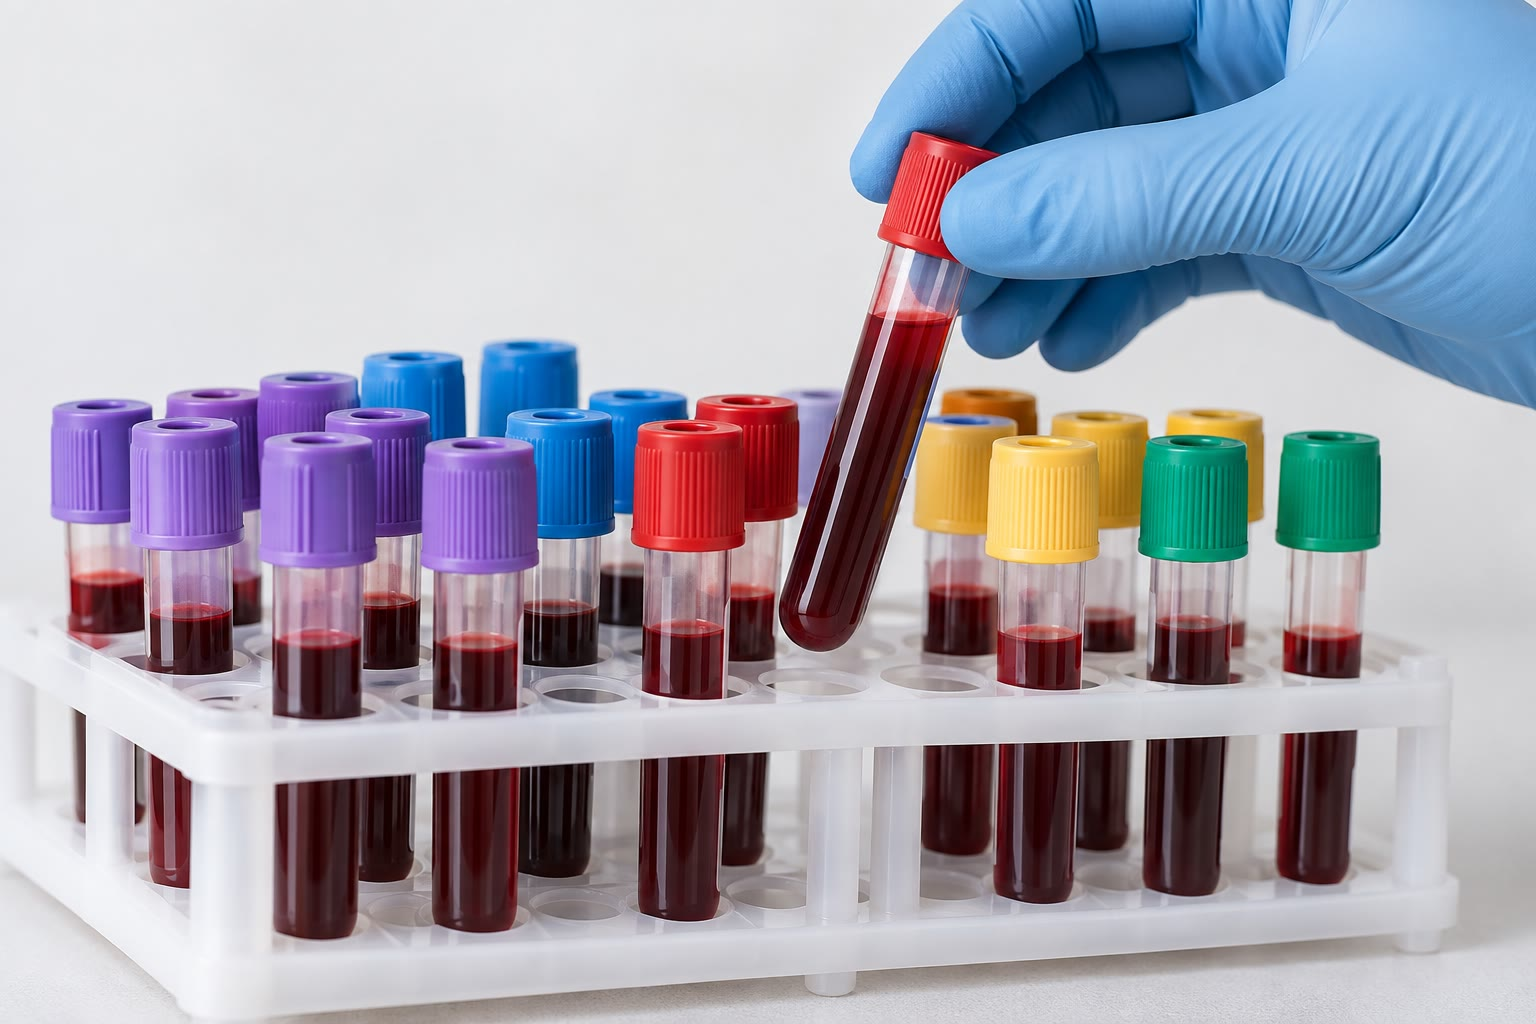
\includegraphics[width=0.45\linewidth]{images/book1/ai/g12-blood-tubes.jpg}

{\small Amostras de sangue: o seu \omterm{def:g9:acids-bases-ph:ph}{pH} é mantido numa faixa estreita.}
\end{omfigure}

\section{Os diagramas de predominância}

\begin{proposition}[A relação de Henderson]\label{prop:g12:buffers-predominance:henderson}
Em qualquer \omterm{def:g6:solutions-and-solubility:solute}{solução aquosa} que contenha o par \ce{HA}/\ce{A-},
\[
  \mathrm{pH} = pK_a + \log\frac{[\ce{A-}]}{[\ce{HA}]} .
\]
\end{proposition}

\begin{proof}
A partir de $K_a = \dfrac{[\ce{A-}][\ce{H3O+}]}{[\ce{HA}]c^\circ}$, tome
$-\log$ dos dois lados: $pK_a = \mathrm{pH} - \log\dfrac{[\ce{A-}]}{[\ce{HA}]}$.
\end{proof}

\begin{definition}[Diagramas de predominância e de distribuição]\label{def:g12:buffers-predominance:predominance}
O \emph{diagrama de predominância}\index{diagrama de predominancia@diagrama de predominância} de um
par é um eixo de \omterm{def:g9:acids-bases-ph:ph}{pH} dividido no $pK_a$: abaixo, predomina o ácido HA
($[\ce{HA}] > [\ce{A-}]$); acima, a base \ce{A-}. O \emph{diagrama de
distribuição}\index{diagrama de distribuicao@diagrama de distribuição} mostra a fração de cada
forma, $[\ce{HA}]/c$ e $[\ce{A-}]/c$, em função do \omterm{def:g9:acids-bases-ph:ph}{pH}; as duas curvas se
cruzam em $\mathrm{pH} = pK_a$.
\end{definition}

\begin{method}[Desenhar um diagrama de predominância]\label{met:g12:buffers-predominance:diagram}
\begin{enumerate}
  \item Desenhe um eixo de \omterm{def:g9:acids-bases-ph:ph}{pH} de 0 a 14 e marque o $pK_a$ do par.
  \item Escreva o ácido à esquerda do $pK_a$ e a base à direita.
  \item Para uma espécie com vários pares (um ácido com dois hidrogênios
        para ceder, um aminoácido), marque todos os $pK_a$: cada
        intervalo pertence a uma forma.
  \item A uma unidade do $pK_a$, a razão já é de 10 para 1: a forma
        minoritária fica abaixo de \qty{10}{\percent}.
\end{enumerate}
\end{method}

\begin{omfigure}
\begin{tikzpicture}[font=\small, x=0.62cm]
  % ledger: pka:ethanoic, pka:methanoic, kb:NH3, ka:H2CO3
  \foreach \y/\pk/\acid/\base in {0/3.74/{\ce{HCOOH}}/{\ce{HCOO-}},
      -1.0/4.76/{\ce{CH3COOH}}/{\ce{CH3COO-}}, -2.0/6.37/{\ce{CO2,H2O}}/{\ce{HCO3-}},
      -3.0/9.26/{\ce{NH4+}}/{\ce{NH3}}} {
    \fill[omThm!20] (0,\y) rectangle (\pk,\y+0.5);
    \fill[omDef!20] (\pk,\y) rectangle (14,\y+0.5);
    \draw[black!50] (0,\y) rectangle (14,\y+0.5);
    \node at (\pk/2,\y+0.25) {\acid};
    \node at ({(\pk+14)/2},\y+0.25) {\base};
    \draw[thick] (\pk,\y-0.08) -- (\pk,\y+0.58);
    \node[font=\scriptsize, anchor=south] at (\pk,\y+0.55) {\pk};
  }
  \draw[->] (0,-3.4) -- (14.5,-3.4) node[right] {pH};
  \foreach \k in {0,2,4,6,8,10,12,14} \draw (\k,-3.35) -- (\k,-3.45) node[below, font=\scriptsize] {\k};
\end{tikzpicture}

{\small \omterm{def:g12:buffers-predominance:predominance}{Diagramas de predominância} de quatro pares: o ácido (à esquerda,
em vermelho) predomina abaixo do seu $pK_a$, a base (à direita, em azul)
acima.}
\end{omfigure}

\begin{omfigure}
\begin{minipage}{0.49\linewidth}
\begin{tikzpicture}
\begin{axis}[width=\linewidth, height=5cm, xmin=0, xmax=14, ymin=0, ymax=1.05,
    xlabel={pH}, ylabel={fração}, axis lines*=left, ymajorgrids,
    grid style={gray!20}, tick label style={font=\scriptsize},
    label style={font=\small}, title={\small ácido etanoico},
    title style={yshift=-4pt}]
  \addplot[very thick, omThm] table[x=pH, y=HA] {figdata/out/grade-12-buffers-predominance-a.dat};
  \addplot[very thick, omDef] table[x=pH, y=A] {figdata/out/grade-12-buffers-predominance-a.dat};
  \addplot[dashed, black!50] coordinates {(4.76,0) (4.76,1)};
  \node[font=\scriptsize, omThm] at (axis cs:2.2,0.85) {\ce{CH3COOH}};
  \node[font=\scriptsize, omDef] at (axis cs:7.6,0.85) {\ce{CH3COO-}};
\end{axis}
\end{tikzpicture}
\end{minipage}\hfill
\begin{minipage}{0.49\linewidth}
\begin{tikzpicture}
\begin{axis}[width=\linewidth, height=5cm, xmin=0, xmax=14, ymin=0, ymax=1.05,
    xlabel={pH}, ylabel={fração}, axis lines*=left, ymajorgrids,
    grid style={gray!20}, tick label style={font=\scriptsize},
    label style={font=\small}, title={\small glicina},
    title style={yshift=-4pt}]
  \addplot[very thick, omThm] table[x=pH, y=cation] {figdata/out/grade-12-buffers-predominance-b.dat};
  \addplot[very thick, omMeth] table[x=pH, y=zwitterion] {figdata/out/grade-12-buffers-predominance-b.dat};
  \addplot[very thick, omDef] table[x=pH, y=anion] {figdata/out/grade-12-buffers-predominance-b.dat};
  \node[font=\scriptsize, omThm] at (axis cs:1.0,0.55) {cátion};
  \node[font=\scriptsize, omMeth] at (axis cs:6.1,0.88) {zwitteríon};
  \node[font=\scriptsize, omDef] at (axis cs:12.6,0.55) {ânion};
\end{axis}
\end{tikzpicture}
\end{minipage}

{\small \omterm{def:g12:buffers-predominance:predominance}{Diagramas de distribuição}, calculados a partir dos valores de
$pK_a$. À esquerda: o ácido etanoico; as curvas se cruzam em 4.76. À
direita: a glicina, \ce{H2N-CH2-COOH}, com dois pares ($pK_a$ 2.35 e
9.78): o \omterm{def:g9:ions:ion}{cátion} \ce{H3N+-CH2-COOH}, o zwitteríon \ce{H3N+-CH2-COO-} e o
\omterm{def:g9:ions:ion}{ânion} \ce{H2N-CH2-COO-}.}
\end{omfigure}

\begin{example}[A glicina no organismo]\label{ex:g12:buffers-predominance:glycine}
% ledger: pka:glycine1, pka:glycine2, ph:blood
No \omterm{def:g9:acids-bases-ph:ph}{pH} do sangue, cerca de 7.4, a glicina fica entre os seus dois valores
de $pK_a$: ela está quase inteiramente na forma de zwitteríon, com uma
carga positiva no nitrogênio e uma carga negativa no carboxilato, neutra
no total. Todos os aminoácidos se comportam da mesma maneira.
\end{example}

\section{Os indicadores ácido--base}


\begin{definition}[Indicador ácido--base, faixa de viragem]\label{def:g12:buffers-predominance:indicator}
Um \emph{indicador ácido--base}\index{indicador acido--base@indicador ácido--base} é um par
\ce{HInd}/\ce{Ind-} cujas duas formas têm cores diferentes, usado em
quantidades muito pequenas. A sua \emph{faixa de
viragem}\index{faixa de viragem} é o intervalo de \omterm{def:g9:acids-bases-ph:ph}{pH} no qual se vê a cor mudar, mais ou menos de
$pK_a - 1$ a $pK_a + 1$: abaixo, vê-se a cor de \ce{HInd}; acima, a de
\ce{Ind-}; e, no meio, uma \omterm{def:g6:pure-substances-and-mixtures:mixture}{mistura} das duas.
\end{definition}

\begin{omfigure}
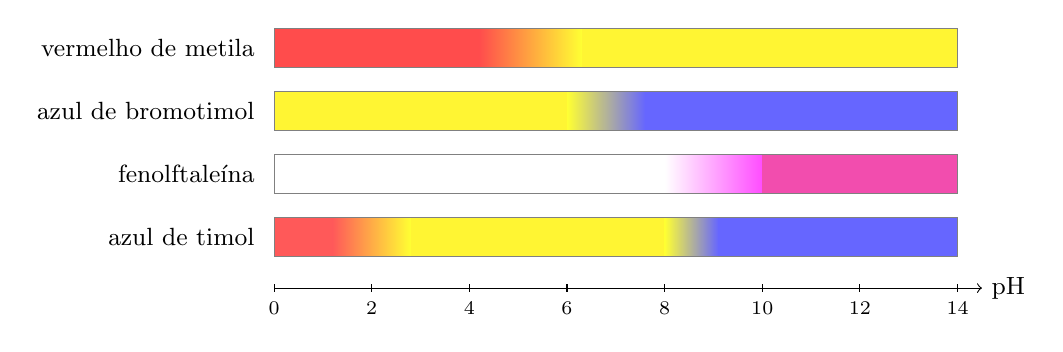
\begin{tikzpicture}[font=\small, x=0.62cm]
  % ledger: ind:methyl-red, ind:BBT, ind:phenolphthalein, ind:thymol-blue, ind:range-rule
  \foreach \y/\name/\a/\b/\ca/\cm/\cb in {
      0/{vermelho de metila}/4.2/6.3/red!70/orange/yellow!80,
      -0.8/{azul de bromotimol}/6.0/7.6/yellow!80/green!60/blue!60,
      -1.6/{fenolftaleína}/8.0/10.0/white/magenta!25/magenta!70} {
    \fill[\ca] (0,\y) rectangle (\a,\y+0.5);
    \shade[left color=\ca, right color=\cb] (\a,\y) rectangle (\b,\y+0.5);
    \fill[\cb] (\b,\y) rectangle (14,\y+0.5);
    \draw[black!50] (0,\y) rectangle (14,\y+0.5);
    \node[anchor=east] at (-0.2,\y+0.25) {\name};
  }
  \fill[red!65] (0,-2.4) rectangle (1.2,-1.9);
  \shade[left color=red!65, right color=yellow!80] (1.2,-2.4) rectangle (2.8,-1.9);
  \fill[yellow!80] (2.8,-2.4) rectangle (8.0,-1.9);
  \shade[left color=yellow!80, right color=blue!60] (8.0,-2.4) rectangle (9.1,-1.9);
  \fill[blue!60] (9.1,-2.4) rectangle (14,-1.9);
  \draw[black!50] (0,-2.4) rectangle (14,-1.9);
  \node[anchor=east] at (-0.2,-2.15) {azul de timol};
  \draw[->] (0,-2.8) -- (14.5,-2.8) node[right] {pH};
  \foreach \k in {0,2,4,6,8,10,12,14} \draw (\k,-2.75) -- (\k,-2.85) node[below, font=\scriptsize] {\k};
\end{tikzpicture}

{\small As cores de quatro indicadores em função do \omterm{def:g9:acids-bases-ph:ph}{pH}; as partes
sombreadas são as \omterm{def:g12:buffers-predominance:indicator}{faixas de viragem}. O azul de timol, com dois pares,
tem duas faixas.}
\end{omfigure}

\begin{method}[Escolher um indicador]\label{met:g12:buffers-predominance:indicator}
Para detectar quando uma solução passa por um dado \omterm{def:g9:acids-bases-ph:ph}{pH} (o \omterm{def:g9:acids-bases-ph:ph}{pH} no fim de
uma \omterm{def:g11:titration:titration}{titulação}, por exemplo), escolha um indicador cuja \omterm{def:g12:buffers-predominance:indicator}{faixa de viragem}
contenha esse \omterm{def:g9:acids-bases-ph:ph}{pH}: a cor muda então exatamente ali.
\end{method}

\section{As soluções-tampão}

\begin{definition}[Solução-tampão]\label{def:g12:buffers-predominance:buffer}
Uma \emph{solução-tampão}\index{solucao-tampao@solução-tampão} é uma solução cujo \omterm{def:g9:acids-bases-ph:ph}{pH}
muda muito pouco quando se acrescenta um pouco de ácido ou de base, ou
quando ela é diluída. Ela é em geral feita de um \omterm{def:g12:ka-and-pka:strong-acid}{ácido fraco} e da sua
base conjugada em quantidades comparáveis; o seu \omterm{def:g9:acids-bases-ph:ph}{pH} fica então próximo
do $pK_a$ do par.
\end{definition}

\begin{proposition}[Por que um tampão resiste]\label{prop:g12:buffers-predominance:buffer}
Num tampão de \ce{HA} e \ce{A-}, um \omterm{def:g12:ka-and-pka:strong-acid}{ácido forte} acrescentado é consumido
pelo \ce{A-} (\ce{A- + H3O+ -> HA + H2O}) e uma \omterm{def:g12:ka-and-pka:strong-acid}{base forte} acrescentada,
pelo \ce{HA} (\ce{HA + OH- -> A- + H2O}); a razão $[\ce{A-}]/[\ce{HA}]$,
e portanto o \omterm{def:g9:acids-bases-ph:ph}{pH}, só muda um pouco. A \omterm{def:g10:concentration-and-dilution:dilution}{diluição} não muda a razão em nada.
\end{proposition}

\begin{proof}
Pela relação de Henderson, o \omterm{def:g9:acids-bases-ph:ph}{pH} só depende da razão. Acrescentar
\qty{1}{mmol} de ácido a um tampão que contém \qty{10}{mmol} de cada
forma muda a razão de $10/10$ para $9/11$, e o \omterm{def:g9:acids-bases-ph:ph}{pH} em apenas
$\log(9/11) = -0.09$.
\end{proof}

\begin{omfigure}
\begin{tikzpicture}
\begin{axis}[width=0.75\linewidth, height=5.6cm, xmin=0, xmax=10, ymin=0,
    ymax=8, xlabel={\ce{HCl} a \qty{0.10}{mol/L} acrescentado (\si{mL})},
    ylabel={pH}, axis lines*=left, ymajorgrids, grid style={gray!20},
    tick label style={font=\small}, label style={font=\small},
    legend style={font=\small, at={(0.98,0.97)}, anchor=north east,
    draw=none, fill=white}, legend cell align=left]
  % ledger: pka:ethanoic (buffer recipe: exercise data)
  \addplot[very thick, omThm, mark=*, mark size=1.3pt] table[x=V, y=water]
    {figdata/out/grade-12-buffers-predominance-c.dat};
  \addplot[very thick, omDef, mark=*, mark size=1.3pt] table[x=V, y=buffer]
    {figdata/out/grade-12-buffers-predominance-c.dat};
  \legend{\qty{100}{mL} de água pura, \qty{100}{mL} de tampão etanoato}
\end{axis}
\end{tikzpicture}

{\small Ácido clorídrico acrescentado à água pura e a um tampão de ácido
etanoico e etanoato de sódio (\qty{0.10}{mol/L} cada um). O \omterm{def:g9:acids-bases-ph:ph}{pH} da água
cai de 7 para cerca de 2; o do tampão, de 4.76 para 4.67.}
\end{omfigure}

\begin{method}[Preparar um tampão]\label{met:g12:buffers-predominance:prepare}
\begin{enumerate}
  \item Escolha um par cujo $pK_a$ esteja a menos de uma unidade do \omterm{def:g9:acids-bases-ph:ph}{pH}
        desejado (de preferência perto dele).
  \item Calcule a razão $[\ce{A-}]/[\ce{HA}] = 10^{\mathrm{pH} - pK_a}$.
  \item \omterm{def:g2:mixing-and-dissolving:mix}{Misture} o \omterm{def:g12:ka-and-pka:strong-acid}{ácido fraco} e um sal da sua base nessa razão, em
        concentrações altas o bastante para absorver as quantidades de
        ácido ou de base.
\end{enumerate}
\end{method}

\begin{inthelab}[Preparar um tampão de pH 4.8]
Misturam-se \qty{50.0}{mL} de ácido etanoico a \qty{0.10}{mol/L} com
\qty{50.0}{mL} de etanoato de sódio a \qty{0.10}{mol/L}; um \omterm{def:g9:acids-bases-ph:ph-paper}{pHmetro}
indica cerca de 4.8. Algumas gotas de ácido clorídrico a
\qty{1}{mol/L} quase não mexem na leitura, enquanto as mesmas gotas em
\qty{100}{mL} de água destilada a fazem cair para cerca de 3.
\end{inthelab}

\section{Os tampões nos seres vivos}

\begin{example}[O tampão do sangue]\label{ex:g12:buffers-predominance:blood}
% ledger: pk:blood-bicarb, ph:blood, hco3:blood
O principal tampão do sangue é o par do dióxido de carbono dissolvido e
do \omterm{def:g9:ions:ion}{íon} hidrogenocarbonato, \ce{CO2,H2O}/\ce{HCO3-}. Para o sangue, os
fisiologistas usam a relação $\mathrm{pH} = 6.1 +
\log\big([\ce{HCO3-}]/[\ce{CO2}]\big)$. Os pulmões eliminam o dióxido de
carbono, os rins ajustam o hidrogenocarbonato: juntos, eles mantêm a
razão e, portanto, o \omterm{def:g9:acids-bases-ph:ph}{pH}.
\end{example}

\begin{omfigure}
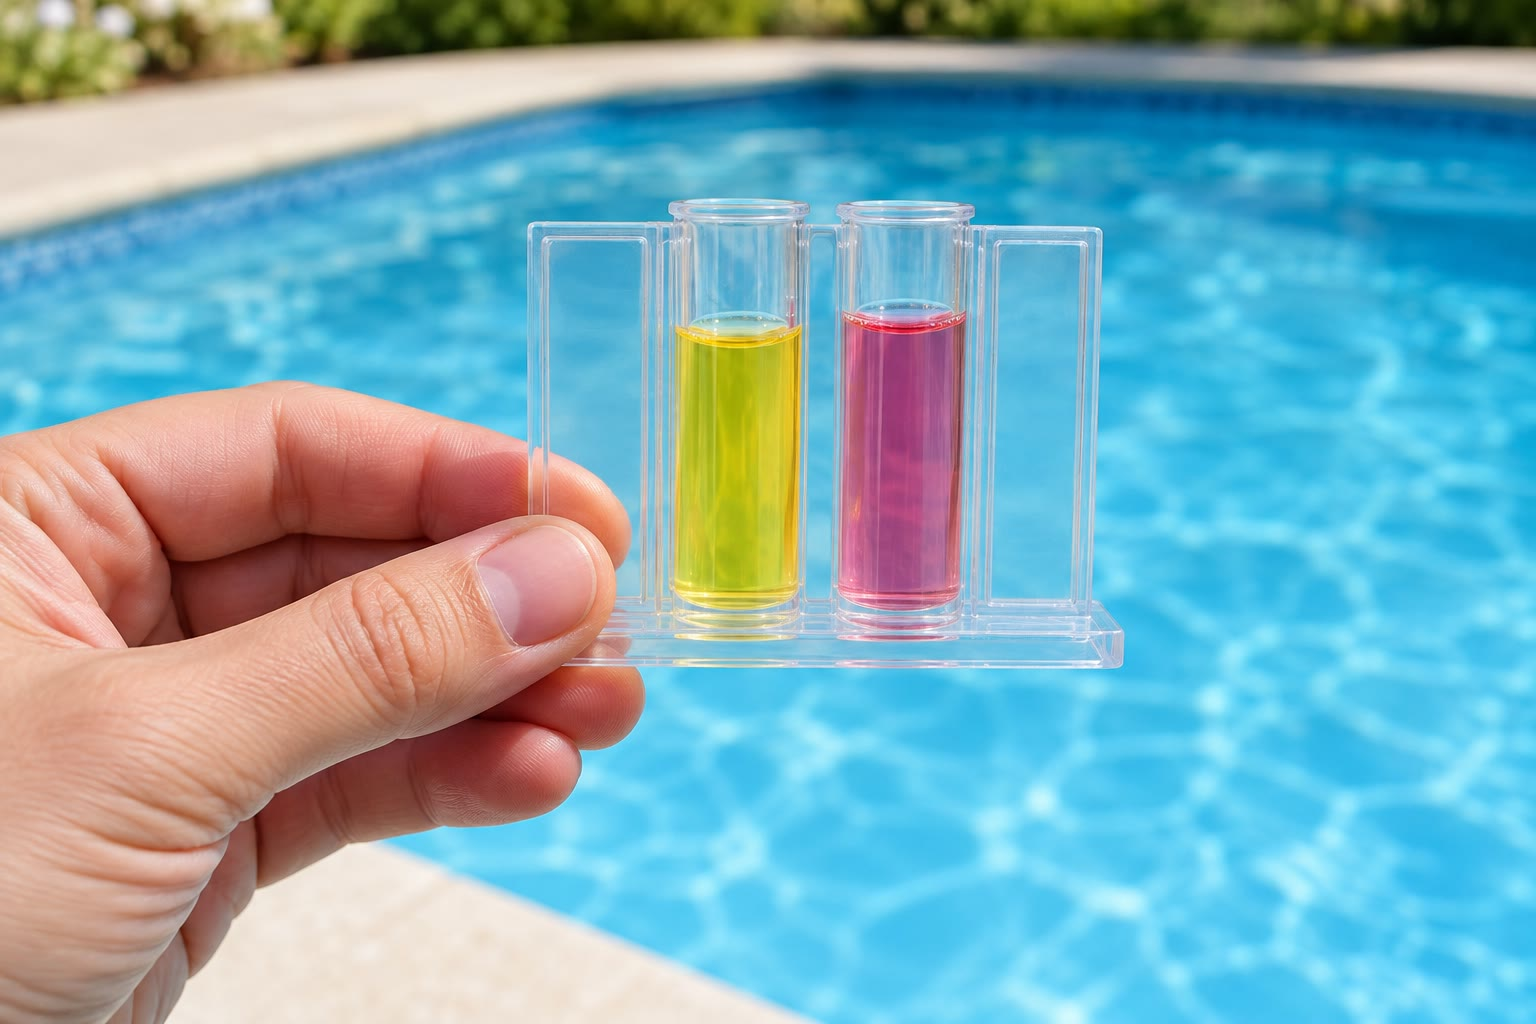
\includegraphics[width=0.45\linewidth]{images/book1/ai/g12-pool-test.jpg}

{\small O teste da água de uma piscina: as cores dos indicadores dão o
\omterm{def:g9:acids-bases-ph:ph}{pH}.}
\end{omfigure}

\section{Exercícios}


\begin{exercise}[$\star$]\label{exo:g12:buffers-predominance:1}
Que forma do par \ce{CH3COOH}/\ce{CH3COO-} ($pK_a = 4.76$) predomina a
\omterm{def:g9:acids-bases-ph:ph}{pH} 2, a \omterm{def:g9:acids-bases-ph:ph}{pH} 4.76 e a \omterm{def:g9:acids-bases-ph:ph}{pH} 7?
\end{exercise}

\begin{exercise}[$\star$]\label{exo:g12:buffers-predominance:2}
No \omterm{def:g12:buffers-predominance:predominance}{diagrama de distribuição} do ácido etanoico, leia a fração de
\ce{CH3COO-} a \omterm{def:g9:acids-bases-ph:ph}{pH} 4 e a \omterm{def:g9:acids-bases-ph:ph}{pH} 6.
\end{exercise}

\begin{exercise}[$\star$]\label{exo:g12:buffers-predominance:3}
Que cor o azul de bromotimol mostra a \omterm{def:g9:acids-bases-ph:ph}{pH} 5? A \omterm{def:g9:acids-bases-ph:ph}{pH} 7? A \omterm{def:g9:acids-bases-ph:ph}{pH} 9?
\end{exercise}

\begin{exercise}[$\star$]\label{exo:g12:buffers-predominance:4}
Que forma do par \ce{NH4+}/\ce{NH3} predomina numa solução de \omterm{def:g9:acids-bases-ph:ph}{pH} 7.4? E
de \omterm{def:g9:acids-bases-ph:ph}{pH} 11?
\end{exercise}

\begin{exercise}[$\star$]\label{exo:g12:buffers-predominance:5}
Por que os indicadores são usados em quantidades muito pequenas?
\end{exercise}

\begin{exercise}[$\star\star$]\label{exo:g12:buffers-predominance:6}
Calcule a razão $[\ce{CH3COO-}]/[\ce{CH3COOH}]$ a \omterm{def:g9:acids-bases-ph:ph}{pH} 3.76, 4.76 e
5.76.
\end{exercise}

\begin{exercise}[$\star\star$]\label{exo:g12:buffers-predominance:7}
Uma \omterm{def:g11:titration:titration}{titulação} termina a \omterm{def:g9:acids-bases-ph:ph}{pH} 8.7. Qual dos quatro indicadores da figura
você escolheria? Por que não o vermelho de metila?
\end{exercise}

\begin{exercise}[$\star\star$]\label{exo:g12:buffers-predominance:8}
Um tampão contém \qty{0.20}{mol/L} de ácido etanoico e
\qty{0.10}{mol/L} de etanoato de sódio. Calcule o seu \omterm{def:g9:acids-bases-ph:ph}{pH}.
\end{exercise}

\begin{exercise}[$\star\star$]\label{exo:g12:buffers-predominance:9}
Usando o diagrama da glicina, dê a forma predominante a \omterm{def:g9:acids-bases-ph:ph}{pH} 1, 6 e 12,
com a sua carga.
\end{exercise}

\begin{exercise}[$\star\star$]\label{exo:g12:buffers-predominance:10}
Leia as curvas de resposta: quanto cai o \omterm{def:g9:acids-bases-ph:ph}{pH} da água depois de
\qty{1.0}{mL} de ácido? E o do tampão?
\end{exercise}

\begin{exercise}[$\star\star$]\label{exo:g12:buffers-predominance:11}
Que par da figura de predominância você escolheria para fazer um tampão
de \omterm{def:g9:acids-bases-ph:ph}{pH} 9.5? Em que razão você misturaria as suas duas formas?
\end{exercise}

\begin{exercise}[$\star\star\star$]\label{exo:g12:buffers-predominance:12}
O tampão etanoato da figura (\qty{10}{mmol} de cada forma) recebe ácido
clorídrico. Quanto ácido ele pode receber antes que o seu \omterm{def:g9:acids-bases-ph:ph}{pH} caia uma
unidade? Por que se diz que um tampão mais concentrado tem uma
capacidade maior?
\end{exercise}

\begin{exercise}[$\star\star\star$]\label{exo:g12:buffers-predominance:13}
Que volume de solução de etanoato de sódio a \qty{0.10}{mol/L} deve ser
acrescentado a \qty{100}{mL} de ácido etanoico a \qty{0.10}{mol/L} para
obter um tampão de \omterm{def:g9:acids-bases-ph:ph}{pH} 5.0?
\end{exercise}

\begin{exercise}[$\star\star\star$]\label{exo:g12:buffers-predominance:14}
O azul de timol tem duas \omterm{def:g12:buffers-predominance:indicator}{faixas de viragem}. Explique por quê, e dê a
sua cor a \omterm{def:g9:acids-bases-ph:ph}{pH} 1, 5 e 10.
\end{exercise}

\begin{exercise}[$\star\star\star$]\label{exo:g12:buffers-predominance:15}
Um tampão de \omterm{def:g9:acids-bases-ph:ph}{pH} 4.76 é diluído dez vezes com água destilada. Qual é o
seu novo \omterm{def:g9:acids-bases-ph:ph}{pH}, segundo a relação de Henderson? O que acontece se um \omterm{def:g12:ka-and-pka:strong-acid}{ácido
forte} de mesmo \omterm{def:g9:acids-bases-ph:ph}{pH} for diluído dez vezes?
\end{exercise}

\section{Problema: o tampão do sangue}

\begin{problem}[{Problema de fim de semana --- que razão entre
hidrogenocarbonato e dióxido de carbono mantém o sangue a pH 7.4?}]
\label{pb:g12:buffers-predominance:1}
% ledger: pk:blood-bicarb, ph:blood, hco3:blood
O \omterm{def:g9:acids-bases-ph:ph}{pH} do sangue arterial fica normalmente entre 7.38 e 7.42. O seu
principal tampão é o par \ce{CO2,H2O}/\ce{HCO3-}, para o qual os
fisiologistas usam $\mathrm{pH} = 6.1 + \log\big([\ce{HCO3-}]/[\ce{CO2}]\big)$.
A concentração normal de hidrogenocarbonato no sangue é de 22 a
\qty{28}{mmol/L}.

\medskip
\noindent\textbf{Parte I --- O par.}
\begin{enumerate}
  \item Escreva a reação do dióxido de carbono dissolvido com a água que
        dá \omterm{def:g9:ions:ion}{íons} hidrogenocarbonato.
  \item Que espécie é o ácido, qual é a base?
  \item O valor 6.1 difere do 6.37 da tabela de $pK_a$. Dê uma razão
        (pense na temperatura do corpo e nos outros \omterm{def:g9:ions:ion}{íons} presentes).
  \item Que \omterm{def:g10:the-mole:amount}{quantidade de matéria} de hidrogenocarbonato contêm
        \qty{5.0}{L} de sangue a \qty{24}{mmol/L}?
\end{enumerate}

\medskip
\noindent\textbf{Parte II --- A predominância.}
\begin{enumerate}[resume]
  \item Desenhe o \omterm{def:g12:buffers-predominance:predominance}{diagrama de predominância} do par com $pK = 6.1$.
  \item Que forma predomina no sangue?
  \item O sangue é levemente ácido ou levemente básico?
\end{enumerate}

\medskip
\noindent\textbf{Parte III --- A razão.}
\begin{enumerate}[resume]
  \item Usando a relação, calcule a razão $[\ce{HCO3-}]/[\ce{CO2}]$ a
        \omterm{def:g9:acids-bases-ph:ph}{pH} 7.4.
  \item Com $[\ce{HCO3-}] = \qty{24}{mmol/L}$, calcule $[\ce{CO2}]$.
  \item Calcule a razão nos dois extremos da faixa normal, 7.38 e 7.42.
  \item Que fração do par está na forma hidrogenocarbonato a \omterm{def:g9:acids-bases-ph:ph}{pH} 7.4?
  \item Um sangue básico demais pode chegar a \omterm{def:g9:acids-bases-ph:ph}{pH} 7.6. Qual é então a
        razão?
\end{enumerate}

\medskip
\noindent\textbf{Parte IV --- Quando o equilíbrio se perde.}
\begin{enumerate}[resume]
  \item Durante um esforço intenso, ácidos entram no sangue. Que forma do
        par os consome? Escreva a reação.
  \item Se o \omterm{def:g9:acids-bases-ph:ph}{pH} caísse para 7.1, qual seria a razão?
  \item Com o hidrogenocarbonato inalterado, quanto o dióxido de carbono
        teria de aumentar? O que fazem os pulmões para reagir?
  \item Por que um \omterm{def:g12:ka-and-pka:strong-acid}{ácido fraco} com a sua base, e não um \omterm{def:g12:ka-and-pka:strong-acid}{ácido forte}, é a
        ferramenta certa para manter um \omterm{def:g9:acids-bases-ph:ph}{pH}?
  \item Quanto o \omterm{def:g9:acids-bases-ph:ph}{pH} muda se as duas concentrações forem divididas por
        dois? Por quê?
  \item Dê a resposta final: qual é a razão entre hidrogenocarbonato e
        dióxido de carbono no sangue a \omterm{def:g9:acids-bases-ph:ph}{pH} 7.4?
\end{enumerate}
\end{problem}
